\newpage
\section{Hamilton-Jacobi Equations \& Calculus of Variation II}
\textbf{Date:} Sep 23, 2021

\subsection{Recap: Connecting H-J equation to calculus of variation via Legendre transform}
Last time, we wanted to compare Hamilton-Jacobi equations to calculus of variations. The
Hamilton-Jacobi equations are of the form
\[
    \left\{\begin{array}{l}
        u_{t}+H(x, \partial u)=0 \quad \text { in } \mathbb{R} \times \mathbb{R}^{n} \\
        u(0)=u_{0} \quad \text { in } \mathbb{R} .
        \end{array}\right.
\]
The characteristics given to this equation are
\[
    \left\{\begin{array}{l}
        \dot{x}=H_{p} \\
        \dot{p}=-H_{x} \\
        \dot{z}=p \cdot H_{p}-H
        \end{array}\right.
\]
with initial data 
\[
\begin{cases}
    x(0) = x_0 \\
    z(0) = u_0\\
    p(0) = \partial_x u_0.
\end{cases}
\]
The first two equations of characteristic system are called the \textbf{Hamilton flow}. In calculus of variations, we have a Lagrangian $L:\RR^n \times \RR^n \to \RR$, and we want to minimize an action functional 
\[
    \min_{x\in \cA} \cL(x) = \min_{x\in \cA} \int_0^T L(x, \dot x)\, dt,
\]
where $\cA = \{x: [0,T] \to \RR \mid x(0)=x_0, x(T) = x_T, x \text{ Lipschitz}\}$. Minimizers satisfy the \textbf{Euler-Lagrange equation}
\[
    L_x(x,\dot x) - \frac{d}{dt}L_q(x, \dot x) =0 .
\]
Last time, we connected these two setups. We saw that $L$ is strictly convex and coercive if and only if $H$ is strictly convex and coercive. And the relation between $H$ and $L$ is 
\[
    H(x, p)=\max _{q \in \mathbb{R}^{n}}-L(x, q)+p \cdot q,
\]
which is maximized at $p=L_q(x,q)$. This relation gives that 
\[
    H(x, p)+L(x, q) \geq p \cdot q
\]
with equality when $p=L_q(x,q)$. This expression is symmetric in $p$ and $q$, so it allows us to cast $q$ in terms of $p: q= H_p(x,p)$. This relationship is known as the \textbf{Legendre tranform}.

\begin{remark}
The Legendre transform is well-defined and is an involution, only assuming convexity.
\end{remark}

\begin{example}
If we remove strict convexity and coercivity, we can get functions which are not defined everywhere. For example, take 
\[
\begin{cases}
    L(0) = 0\\
    L(q)= -\infty \quad q \neq 0
\end{cases}
\]
What is $H$ in this case?
\end{example}

We have not incorporated the initial data of the Hamilton-Jacobi equations into our
calculus of variations. We will do this by adding $u_0(x_0)$ to the minimization problem (so when $T=0$, we get $u_0(x_0)$ and removing the condition $x(0)=x_0$ from our set $\cA$. So we are minimizing 
\begin{equation}
    \label{eq: E-L}
    \min _{x \in \mathcal{A}} \int_{0}^{T} L(x, \dot{x}) d t+u_{0}\left(x_{0}\right)=u\left(T, x_{T}\right),
\end{equation}
with $\cA = \{x: [0,T] \to \RR \text{ Lipschitz}| x(T) = x_T\}$.

\subsection{Existence of minimizers for the Euler-Lagrange equation}
We want to prove:
\begin{theorem}
    The minimal value function $u(T, x_T)$ in teh calculus of variations is the solution to the H-J equations
\end{theorem}

First, we should ask: Does a minimum solution to the Euler-Lagrange equation exist? The answer is yes, as long as $L$ is convex, coercive, and Lipschitz in $x$ and if $u_0\in \Lip$. However, there is no guarantee of uniqueness. We will not prove this, but here is some intuition: 

Here is  the trivial case: 
\begin{proposition}
    SUppose we have a continuous function $F:K\to \RR$ with $K$ compact. Then $\min F$ is attained.
\end{proposition}
\begin{proof}
    Just consider the campactness of $K$. \qed 
\end{proof}

What if we try to apply this to calculus of variations? Suppose we have a minimizing
sequence $x_n:[0,T] \to \RR^n$. Then $\cL(x_n) \to u(T, x_T)$ but in what topology? Is $x_n$ in a bounded set? We know that $\cL(x_n)$ is bounded. If$L(x,q) = q^2$, for example, we could conclude that $\int_0^T(\dot x_n)^2 \le c$. Then $\dot x_n$ is bounded in $L^2([0,T])$. This would imply that $x_n$ is bounded in $C^{1/2}$ using Holder's inequality: ($|x_n(t)-x_n(s)|\le c|t-s|^{1/2}$).  This implies that $x_n$ is equicontinuous (and equibounded by the $x(T) = x_T$ assumption). So the Arzela-Ascoli theorem says that $x_n \to x$ uniformly ($x_n$ is a subsequence). Then 
\[
    \lim_{n\to \infty} \cL(x_n) = \lim_{n\to \infty}\int_0^TL(x_n, \dot x_n) dt + u(x_n,0)
\]
We can pas to the limit without a problem for $x$, but the convergence with respect to $\dot x$ is trouble. The limit of the intergral may not exist, but maybe we can hope for 
\[
    \int_{0}^{T} L(x, \dot{x}) d t \leq \liminf _{n \rightarrow \infty} \int_{0}^{T} L\left(x_{n}, \dot{x}_{n}\right) d t
\]
This is lower seminicountinuity for the map $x\to \cL(x)$.The key observation is that convexity of $\cL$ implies lower semicontinuity of $\cL$.

\begin{proposition}
    The minimum solution to the Euler-Lagrange equation \eqref{eq: E-L} exists.
\end{proposition}
\begin{proof}
    The convexity inequality tells us that 
    \[
        L(\dot x_n) \ge L(\dot x) + L_q(\dot x) (\dot x_n-\dot x).
    \]
    Integrating gives us 
    \[
        \int_0^T L(\dot x_n) \, dt \ge \int_0^T L(\dot x) dt + \int_0^T L_q(\dot x)(\dot x - \dot x_n) dt.
    \]
    We are done if $\lim_{n\to \infty}\int L_q(\dot x) (\dot x_n - \dot x) =0$. We ahve replaced our nonlinear dependence on $\dot x_n - \dot x$ by a linear property. Since $\dot x \in L^2$, we can approxiamte $L_q(\dot x)$ by smooth functions. Suppose $y_k\in \con^\infty$ with $y_k\to L(\dot x)$ in $L^2$. It's enough to see that 
    \[
        \lim _{n \rightarrow \infty} \int_{0}^{T} y_{k}\left(\dot{x}_{n}-\dot{x}\right) d t=0
    \]
    In this context, we can integrate by parts. The integral equals 
    \[
        \int_{0}^{T} y_{k}\left(\dot{x}_{n}-x\right) d t=\int_{0}^{T} \dot{y}_{k}\left(x_{n}-x\right) d t+\left.y_{k}\left(x_{n}-x\right)\right|_{0} ^{T} \stackrel{n \rightarrow \infty}{\longrightarrow} 0
    \]
    by uniform convergence of $x_n \to x$. 
    \qed 
\end{proof}

\begin{example}
Recall our double well potential
\begin{figure}[H]
    \centering
    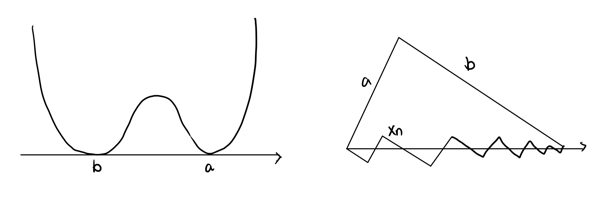
\includegraphics[width=0.8\textwidth]{pics/9-1.png}
\end{figure}
In this case, if $x_n$ is a wiggle approximating the $0$ trajectory, we have $\cL(\dot x_n)=0$ by $\cL(\dot(x)) = \cL(0) >0$.
\end{example}

\begin{remark}
    The Hamilton-Jacobi equation can be solved for a short time using characteristics. In calculus of variations, the analogue turns out to be that minimizers are unique for a short time.
\end{remark}

We want to think of two minimizers in calculus of variations as characteristics that interect. 
\begin{figure}[H]
    \centering
    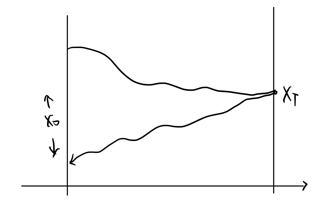
\includegraphics[width=0.7\textwidth]{pics/9-2.png}
\end{figure}
\subsection{E-L equation minimizers slove H-J equations}
\vspace{1em}
\begin{proof}
    Suppose $x$ is a minimizer for the action functional. We can choose a intermediate
point $t$, and first minimize relative to the time $t$.

\begin{figure}[H]
    \centering
    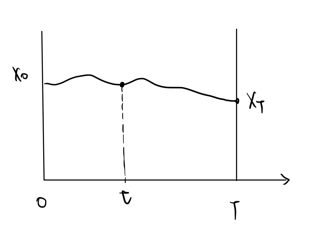
\includegraphics[width=0.7\textwidth]{pics/9-3.png}
\end{figure}

\[
    \min _{x} \int_{0}^{T} L(x, \dot{x}) d t+u_{0}\left(x_{0}\right)=\min _{x} \int_{0}^{t} L(x, \dot{x}) d s+u_{0}\left(x_{0}\right)+\int_{t}^{T} L(x, \dot x) d s
\]
If $\left.x\right|_{[0, T]}$ is a minimizer, then $\left.x\right|_{[0, t]}$ is also a minimizer. So
$$
u\left(x_{T}, x_{0}\right)=\min u\left(x_{t}, x_{0}\right)+\int_{t}^{T} L(x, \dot{x}) d s
$$
This is called the \textbf{Dynamic programming principle}. This principle tells us that for minimizers, 
\[
    u\left(x_{T}, x_{0}\right)=u\left(x_{t}, x_{0}\right)+\int_{t}^{T} L(x, \dot{x}) d s
\]
which we can differentiate with respect to $t$ to get
$$
\begin{aligned}
\frac{d}{d t} u\left(x_{t}, x_{0}\right) &=L(x, \dot{x}) \\
&=p \cdot q-H(x, p) \\
&=p \cdot H_{p}-H
\end{aligned}
$$
We conclude that $u\left(t, x_{t}\right)$ from the calculus of variations is the same as the $u\left(t, x_{t}\right)$ from the Hamilton-Jacobi equation because they solve the same equation with the same initial data at time $0 .$ \qed 
\end{proof}

\begin{remark}
    This is not an entirely correct proof. How do we know that there is an
optimal trajectory starting at $x_0$? If the time is short enough, we can guarantee a minimizer
starting at $x_0$, but this is exactly the issue of uniqueness of minimizers. This proof can be
made rigorous for short times.

\end{remark}

\begin{remark}
More generally, this is related to control theory, where we try to find 
\[
    u(x_0, T) = \min  \int_0^T L(x,f)dt + u_0(x(0)), \quad \dot x = h(x,f).
\]
Here we chan choose some weight of influence by changing $f$ and we are trying to optimize some cost functional. The function $u(x_0, T)$ solves a H-J equation. We can think of our claculus of variations problem as the case where the ODE for $x$ is given by $\dot x = f$.
\end{remark}

\begin{remark}
    Calculus of variation allows us to obtain meaning solutions for H-J equations after characteristics to intersect. Instead of picking which characteristic to continue, we can just  look for a minimizer for a calculus of variations problem in longer time.
\end{remark}
